\section{Stator redesign: Wave}
\label{Chap:stator_redesign}
Using the problem analysis in Chapter \ref{Chap:stator_analysis}, some changes have been made to reduce the stresses of the stator during operational and shut-down conditions. The changes are made based on the RPCs (see Appendix \ref{AppendixF}), considering all requirements, constraints and preferences. This chapter will address which changes are made, why they are made, and what effect the change has for the stresses. Then, the results for both conditions will be given. In Figure \ref{fig:final_stator}, the re-designed stator is shown, where the numbers indicate an area where a change was made to the original stator.
\begin{figure}[H]
\centering
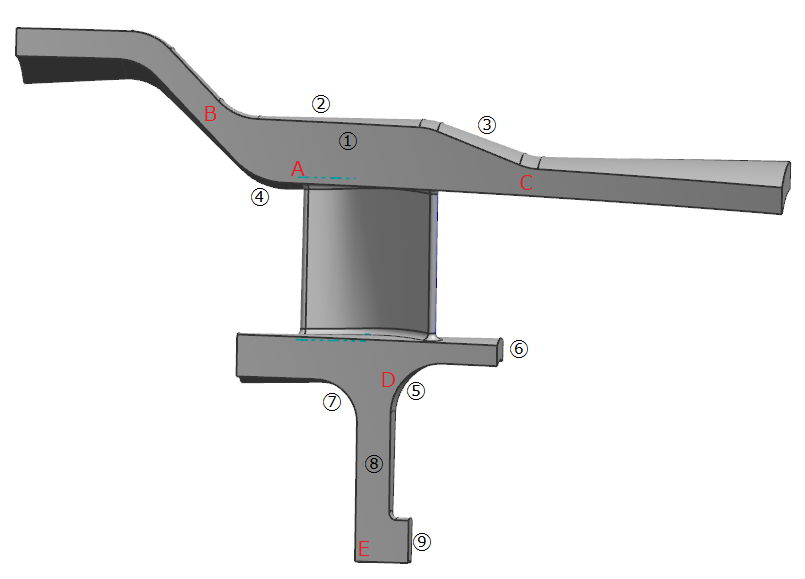
\includegraphics[width=0.8\textwidth]{Figures/final_stator.png}
\caption{The re-designed stator with the indicated changes (1,2,..,9) and high stress points (A,B,..,E).}
\label{fig:final_stator}
\end{figure}
A design is made which is called the 'wave'. Due to its shape, the temperature gradient is lower around the blade-stator transition, where originally the highest stress occurred during the shut-down condition \cite{temperaturepressure}. The high stress points during the operating conditions are related to the shape of the bottom. The bigger edges and thicker planes are successful in lowering the stress. 

\subsection{Description of changes}
\begin{enumerate}
\item The wave itself can be adapted in three dimensions: the length (1), height (2) and angle (3). As said, the temperature gradient will be lower in the blade-stator transition (A), but the wave creates higher stress in the diagonal part (B) and beneath the angle (C). Due to the deformation around these points, the stresses will increase. 
\item The curve in point (4) is moved towards the blade-stator transition; this is done in order to create a larger angle in the diagonal part.
\item To reduce the stress in the lower part of the stator (in operating condition), the temperature gradient must be lowered in and around the edge blend. This is done by increasing the radius of the edge blend in point (5).
\item The beam connected to the edge blend (6) is made a little thicker, which will lower the very high temperature gradient in this part. By lowering the gradient, the deformation will be less, and, therefore, the stress in the edge blend will be lowered.
\item The vertical tail part (8) has been moved towards the center below the blade; this is done in order to create a larger possible radius for the edge blend.
\item The radius of the edge blend in point (7) increased as well; this is again done to lower the temperature gradient at this point.
\item The last change is made to the lid (9), which is reversed in comparison to the original stator. This change is based on the air flow that the stator will endure. There will be less pressure on the vertical tail part, because the air will not get stuck in the 'bowl' created by the lid, tail and surface beneath the blade, since the air will flow from the left looking at Figure \ref{fig:final_stator}.
\end{enumerate}
A FEM analysis will be applied to the redesign of the stator; the results can be seen in Chapter \ref{Results}. An alternative design that is investigated but eliminated can be found in Appendix \ref{AppendixA3}.

\subsection{Compatibility \& Functionality}
As mentioned in the RPCs (Appendix \ref{AppendixF}), the stator is constrained to remain functional and compatible with the stator. Therefore, the 'wave' design should comply with these constraints; otherwise, it can not be used for a jet engine. The compatibility requires that the total jet engine can be assembled correctly with the newly designed stator. Figure \ref{fig:compatible} shows the position of the stator in the jet engine.
\begin{figure}[H]
\centering
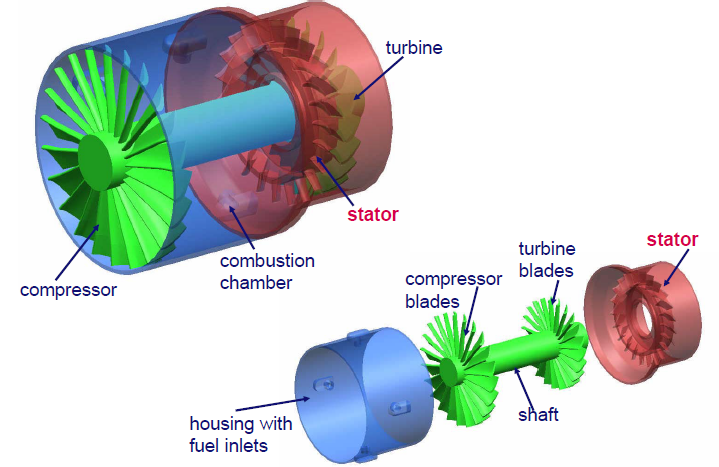
\includegraphics[width=0.6\textwidth]{Figures/compatible.png}
\caption{The compatibility of the stator in the total jet engine and in an exploded view \cite{COC}}
\label{fig:compatible}
\end{figure}
The 'wave' design stator can be compared with the stator in the figure shown above. As you can see, there is not much of a change in the contact area between the stator and the compressor shaft or housing. Therefore, it can be concluded that the 'wave' design remains compatible.

The functionality constraint states that the stator should still be able to convert the increased rotational kinetic energy, caused by the blade, into static pressure. According to the 4GC00 COC, which included Figure \ref{orange outline}, it is not allowed to make adjustments to the blade \cite{COC}. In addition, the surface around the blade, which is in contact with the inflowing air, is barely changed. This means that the functionality will not change with the original stator. The 'wave' design agrees with both the compatibility and functionality constraint.  
\newpage